%%%%%%%%%%%%%%%%%%%%%%%%%%ch3-3
\begin{frame}[shrink]
  \frametitle{ch3.信号检测与估计理论的基础知识}
  \framesubtitle{ch3-3. M元信号的统计检测及参量信号的统计检测}
  \tableofcontents[hideallsubsections]
\end{frame}

\section{M元信号的统计检测}

\begin{frame}{M元信号的统计检测}
\begin{block}{基本要求}
	\begin{itemize} \setstretch{2.5}
		\item 了解贝叶斯准则
		\item 了解最小平均错误概率准则和最大似然准则
	\end{itemize}
\end{block}
\end{frame}

\begin{frame}{M元信号检测检测模型}
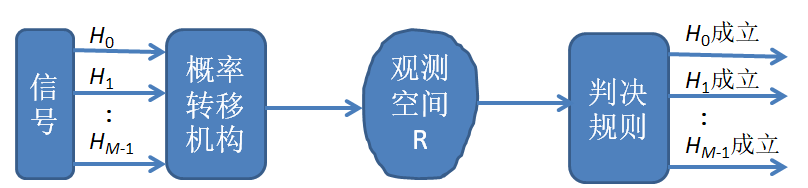
\includegraphics[scale=0.4]{M}
\newline
\begin{columns}
\column{0.4\textwidth}
判决域划分:
\[\bm{R}=\bigcup_{i=0}^{M-1}R_i, R_i\cap R_j=\emptyset, (i\ne j) \]
\column{0.6\textwidth}
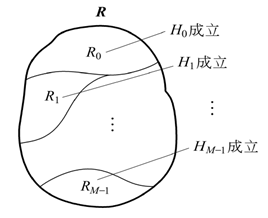
\includegraphics[scale=0.4]{R-M}
\end{columns}
\end{frame}

\begin{frame}[shrink]{贝叶斯准则}
给定各假设先验概率及各判决代价因子。问题: 寻找一种判决空间的划分方法, 使平均代价最小。\\
\textbf{平均代价: }
\begin{align*}
C&=P(H_0)C(H_0)+P(H_1)C(H_1)\\
C(H_0)&=c_{00}P(H_0|H_0)+c_{10}P(H_1|H_0)\\
C(H_1)&=c_{01}P(H_0|H_1)+c_{11}P(H_1|H_1)\\
C=&P(H_0)(c_{00}P(H_0|H_0)+c_{10}P(H_1|H_0))+\\
&P(H_1)(c_{01}P(H_0|H_1)+c_{11}P(H_1|H_1))
\end{align*}
\centering$\Downarrow$
\[
C=\sum_{i=0}^{M-1}\sum_{j=0}^{M-1}c_{ij}P(H_j)P(H_i|H_j)
\]
\end{frame}

\begin{frame}[shrink]{平均代价计算}
\begin{align*}
C&=\sum_{i=0}^{M-1}\sum_{j=0}^{M-1}c_{ij}P(H_j)P(H_i|H_j)\\
&=\sum_{i=0}^{M-1}c_{ii}P(H_i)P(H_i|H_i)+\sum_{i=0}^{M-1}\sum_{j=0,j\ne i}^{M-1}c_{ij}P(H_j)P(H_i|H_j)\\
&\quad \text{by } P(H_i|H_i)=1-\sum_{j=0,j\ne i}^{M-1}P(H_j|H_i)\\
&=\sum_{i=0}^{M-1}c_{ii}P(H_i)\left(1-\sum_{j=0,j\ne i}^{M-1}P(H_j|H_i)\right)+\sum_{i=0}^{M-1}\sum_{j=0,j\ne i}^{M-1}c_{ij}P(H_j)P(H_i|H_j)\\
&=\sum_{i=0}^{M-1}c_{ii}P(H_i)-\sum_{i=0}^{M-1}\sum_{j=0,j\ne i}^{M-1}c_{ii}P(H_i)P(H_j|H_i)+\sum_{i=0}^{M-1}\sum_{j=0,j\ne i}^{M-1}c_{ij}P(H_j)P(H_i|H_j)\\
\end{align*}
\end{frame}

\begin{frame}[shrink]{平均代价计算}
\begin{align*}
&\text{因为 }\quad \sum_{i=0}^{M-1}\sum_{j=0}^{M-1}c_{ii}P(H_i)P(H_j|H_i)=\sum_{i=0}^{M-1}\sum_{j=0}^{M-1}c_{jj}P(H_j)P(H_i|H_j)\\
&\text{所以 }\quad \sum_{i=0}^{M-1}\sum_{j=0,j\ne i}^{M-1}c_{ii}P(H_i)P(H_j|H_i)=\sum_{i=0}^{M-1}\sum_{j=0,j\ne i}^{M-1}c_{jj}P(H_j)P(H_i|H_j)
\end{align*}
\begin{align*}
C&=\sum_{i=0}^{M-1}c_{ii}P(H_i)-\sum_{i=0}^{M-1}\sum_{j=0,j\ne i}^{M-1}c_{ii}P(H_i)P(H_j|H_i)+\sum_{i=0}^{M-1}\sum_{j=0,j\ne i}^{M-1}c_{ij}P(H_j)P(H_i|H_j)\\
&=\sum_{i=0}^{M-1}c_{ii}P(H_i)+\sum_{i=0}^{M-1}\sum_{j=0,j\ne i}^{M-1}\left(c_{ij}-c_{jj}\right)P(H_j)P(H_i|H_j)\\
&=\sum_{i=0}^{M-1}c_{ii}P(H_i)+\sum_{i=0}^{M-1}\int_{R_i}\sum_{j=0,j\ne i}^{M-1}\left(c_{ij}-c_{jj}\right)P(H_j)p(\bm{x}|H_j)d\bm{x}\\
\end{align*}
\end{frame}

\begin{frame}[shrink]{贝叶斯准则}
\begin{align*}
C=\sum_{i=0}^{M-1}c_{ii}P(H_i)+\sum_{i=0}^{M-1}\int_{R_i}\sum_{j=0,j\ne i}^{M-1}\left(c_{ij}-c_{jj}\right)P(H_j)p(\bm{x}|H_j)d\bm{x}
\end{align*}
\begin{align*}
I_{i}(\bm{x})=\sum_{j=0,j\ne i}^{M-1}\left(c_{ij}-c_{jj}\right)P(H_j)p(\bm{x}|H_j)
\end{align*}
\[c_{ij}\ge c_{jj},\quad P(H_j)\ge 0,\quad p(\bm{x}|H_j)\ge 0\implies I_{i}(\bm{x})\ge 0 \]
\begin{block}{贝叶斯准则}
为保证平均风险最小,应把所有使$I_{i}(\bm{x})$最小的$\bm{x}$划分至$R_i$判决区域,即当满足
\[I_{i}(\bm{x})<I_j(\bm{x}), j=0,1,\cdots,M-1, j\ne i \]
时, 判决$H_i$成立
\[R_i=\{\bm{x}|I_i(\bm{x})<I_j(\bm{x}), 0\le j\le M, j\ne i\} \]
\end{block}
\end{frame}

\begin{frame}[shrink]{贝叶斯准则}
\begin{block}{贝叶斯准则}
为保证平均风险最小,应把所有使$I_{i}(\bm{x})$最小的$\bm{x}$划分至$R_i$判决区域,即当满足
\[I_{i}(\bm{x})<I_j(\bm{x}), j=0,1,\cdots,M-1, j\ne i \]
时, 判决$H_i$成立
\[R_i=\{\bm{x}|I_i(\bm{x})<I_j(\bm{x}), 0\le j\le M, j\ne i\} \]
\end{block}
\begin{block}{$H_0$成立的判决域, 是满足下列方程组的解}
\[
\begin{cases}
I_0(\bm{x})< I_1(\bm{x})\\
I_0(\bm{x})< I_2(\bm{x})\\
\hspace{1cm} \vdots\\
I_0(\bm{x})< I_{M-1}(\bm{x})
\end{cases}
\]
\end{block}
\end{frame}

\begin{frame}[shrink]{贝叶斯准则}
\textbf{\textcolor{blue}{定义似然比函数}}
\[\lambda_i(\bm{x})=\frac{p(\bm{x}|H_i)}{p(\bm{x}|H_0)}, \quad i=0,1,\cdots,M-1 \]
\[J_i(\bm{x})=\frac{I_i(\bm{x_i})}{p(\bm{x}|H_0)}=\sum_{j=0,j\ne i}^{M-1}P(H_j)(c_{ij}-c_{jj})\lambda_i(\bm{x}), \quad i=0,1,\cdots,M-1 \]
\textbf{\textcolor{blue}{定义判决规则}}\\
~\\
如果
\[J_i(\bm{x})<J_j(\bm{x})\quad (j=0,1,\cdots,M-1,j\ne i)\]
则判决$H_i$成立
\end{frame}

\begin{frame}[shrink]{最小平均错误准则}
\begin{align*}
&C=\sum_{i=0}^{M-1}c_{ii}P(H_i)+\sum_{i=0}^{M-1}\int_{R_i}\sum_{j=0,j\ne i}^{M-1}\left(c_{ij}-c_{jj}\right)P(H_j)p(\bm{x}|H_j)d\bm{x}\qquad I_{i}(\bm{x})=\sum_{j=0,j\ne i}^{M-1}\left(c_{ij}-c_{jj}\right)P(H_j)p(\bm{x}|H_j)\\
&\text{正确判决代价为0, 错误判决代价为1的条件下: }\quad I_{i}(\bm{x})=\sum_{j=0,j\ne i}^{M-1}P(H_j)p(\bm{x}|H_j)
\end{align*}
\begin{block}{最小平均错误准则}
为保证最小错误概率,应把所有使$I_{i}(\bm{x})$最小的$\bm{x}$划分至$R_i$判决区域,即当满足
\[I_{i}(\bm{x})<I_j(\bm{x}), j=0,1,\cdots,M-1, j\ne i \]
时, 判决$H_i$成立
\[R_i=\{\bm{x}|I_i(\bm{x})<I_j(\bm{x}), 0\le j\le M, j\ne i\} \]
\end{block}
\begin{align*}
&\textbf{\textcolor{blue}{最小平均错误概率:}}\quad P_e=\sum_{i=0}^{M-1}\sum_{j=0}^{M-1}P(H_j)P(H_i|H_j),\quad j\ne i
\end{align*}
\end{frame}

\begin{frame}[shrink]{最小平均错误准则}
$H_0$成立的判决域, 是满足下列下面方程组的解
\[
\begin{cases}
I_0(\bm{x})< I_1(\bm{x})\\
I_0(\bm{x})< I_2(\bm{x})\\
\hspace{1cm} \vdots\\
I_0(\bm{x})< I_{M-1}(\bm{x})
\end{cases}
\]
$H_1$成立的判决域, 是满足下列下面方程组的解
\[
\begin{cases}
I_1(\bm{x}) < I_0(\bm{x})\\
I_1(\bm{x}) < I_2(\bm{x})\\
\hspace{1cm} \vdots\\
I_1(\bm{x}) < I_{M-1}(\bm{x})
\end{cases}
\]
\end{frame}

\begin{frame}[shrink]{最大似然准则}
\begin{align*}
&C=\sum_{i=0}^{M-1}c_{ii}P(H_i)+\sum_{i=0}^{M-1}\int_{R_i}\sum_{j=0,j\ne i}^{M-1}\left(c_{ij}-c_{jj}\right)P(H_j)p(\bm{x}|H_j)d\bm{x}\\ &I_{i}(\bm{x})=\sum_{j=0,j\ne i}^{M-1}\left(c_{ij}-c_{jj}\right)P(H_j)p(\bm{x}|H_j)\\
&\textbf{\textcolor{blue}{正确判决代价为0,错误判决代价为1,且信源的假设先验概率相等: }} P(H_j)=\frac{1}{M} \\
&I_{i}(\bm{x})=\sum_{j=0,j\ne i}^{M-1}P(H_j)p(\bm{x}|H_j)=\frac{1}{M}\sum_{j=0,j\ne i}^{M-1}p(\bm{x}|H_j)=\frac{1}{M}\left(\sum_{j=0}^{M-1}p(\bm{x}|H_j)-p(\bm{x}|H_i)\right)
\end{align*}
\textbf{\textcolor{blue}{判决规则是M个似然函数$p(\bm{x}|H_i), i=0,1,\cdots,M-1$中, 选择使$p(\bm{x}|H_i)$最大的假设成立}}
\begin{align*}
&\textbf{\textcolor{blue}{最小平均错误概率:}}\quad P_e=\sum_{i=0}^{M-1}\sum_{j=0}^{M-1}P(H_j)P(H_i|H_j)=\frac{1}{M}\sum_{i=0}^{M-1}\sum_{j=0}^{M-1}P(H_i|H_j),\quad j\ne i
\end{align*}
\end{frame}

\begin{frame}[shrink]{最大似然准则}
$H_0$成立的判决域, 是满足下列下面方程组的解
\[
\begin{cases}
p(\bm{x}|H_0)> p(\bm{x}|H_1)\\
p(\bm{x}|H_0)> p(\bm{x}|H_2)\\
\hspace{1cm} \vdots\\
p(\bm{x}|H_0)> p(\bm{x}|H_{M-1})\\
\end{cases}
\]
$H_1$成立的判决域, 是满足下列下面方程组的解
\[
\begin{cases}
p(\bm{x}|H_1)> p(\bm{x}|H_0)\\
p(\bm{x}|H_1)> p(\bm{x}|H_2)\\
\hspace{1cm} \vdots\\
p(\bm{x}|H_1)> p(\bm{x}|H_{M-1})\\
\end{cases}
\]
\end{frame}

\begin{frame}{M元信号检测例题8}
例8:在四元通信系统中,信源有四个可能的输出,即假设为$H_0$时输出1,假设为$H_1$时输出为2,假设为$H_2$时输出为3,假设为$H_3$时输出为4。各个假设的先验概率相等,且正确判决代价为0,错误判决代价为1,并进行了N次独立观测。
信号在传输过程中叠加有均值为零,方差为$\sigma_n^2$的加性高斯白噪声。\\
~\\
试设计一个四元信号的最佳检测系统。
\end{frame}

\begin{frame}{M元信号检测例题9}
在三元通信系统中,信源有三个可能的输出,即假设为$H_0$时输出$-A$,假设为$H_1$时输出为0,假设为$H_2$时输出为$A$。各个假设的先验概率相等,且正确判决代价为0,错误判决代价为1,并进行了$N$次独立观测。
信号在传输过程中叠加有均值为零,方差为$\sigma_n^2$的加性高斯白噪声。\\
~\\
试按照最小平均错误概率准则设计检测系统,并求正确判决和错误判决的概率。
\end{frame}

\begin{frame}[shrink]{M元信号检测例题9: 解}
解: 本例的检测模型为:
\begin{align*}
&H_0: x_k=-A+n_k\\
&H_1: x_k=n_k\\
&H_2: x_k=A+n_k
\end{align*}
根据题设: 各个假设的先验概率相等,且正确判决代价为0,错误判决代价为1。\\
因此本例的贝叶斯检测等价于最大似然检测,即使似然函数$p(\bm{x}|H_i)$最大的观测值划分个判决区域$R_i$.
\end{frame}

\begin{frame}[shrink]{M元信号检测例题9: 解续(1)}
\textbf{\textcolor{blue}{步骤1: 计算各假设下的似然函数}}\\
~\\
由于$n_k$是高斯分布随机变量, 因此在$H_0$假设下, 第$k$次采样值$x_k$服从高斯分布,且均值为$-A$, 方差为$\sigma_n^2$; 在$H_1$假设下, 第$k$次采样值$x_k$服从均值为0, 方差为$\sigma_n^2$的高斯分布; 在$H_2$假设下, 第$k$次采样值$x_k$服从均值为$A$, 方差为$\sigma_n^2$的高斯分布。
\scriptsize
\begin{align*}
p(x_k|H_0)&=\left(\frac{1}{2\pi\sigma_n^2}\right)^{1/2}\exp\left(-\frac{(x_k+A)^2}{2\sigma_n^2}\right)
&\implies& p(\bm{x}|H_0)=\prod_{k=1}^{N}\left(\frac{1}{2\pi\sigma_n^2}\right)^{1/2}\exp\left(-\frac{(x_k+A)^2}{2\sigma_n^2}\right)\\
p(x_k|H_1)&=\left(\frac{1}{2\pi\sigma_n^2}\right)^{1/2}\exp\left(-\frac{x_k^2}{2\sigma_n^2}\right)&\implies& p(\bm{x}|H_1)=\prod_{k=1}^{N}\left(\frac{1}{2\pi\sigma_n^2}\right)^{1/2}\exp\left(-\frac{x_k^2}{2\sigma_n^2}\right)\\
p(x_k|H_2)&=\left(\frac{1}{2\pi\sigma_n^2}\right)^{1/2}\exp\left(-\frac{(x_k-A)^2}{2\sigma_n^2}\right)&\implies& p(\bm{x}|H_2)=\prod_{k=1}^{N}\left(\frac{1}{2\pi\sigma_n^2}\right)^{1/2}\exp\left(-\frac{(x_k-A)^2}{2\sigma_n^2}\right)
\end{align*} 
\normalsize
\begin{align*}
&\textbf{以上3个似然函数统一写成:} \quad p(\bm{x}|H_i)=\prod_{k=1}^{N}\left(\frac{1}{2\pi\sigma_n^2}\right)^{1/2}\exp\left(-\frac{(x_k-s_i)^2}{2\sigma_n^2}\right),\quad i=0,1,2\\
&\text{其中,} \quad s_0=-A\qquad s_1=0\qquad s_2=A
\end{align*}
\end{frame}

\begin{frame}[shrink]{M元信号检测例题9: 解续(2)}
\textbf{\textcolor{blue}{步骤2: 按照最大似然准则划分观测空间}}
%\small
\begin{columns}[T]
\column{0.5\textwidth}
\begin{align*}
p(\bm{x}|H_i)&=\prod_{k=1}^{N}\left(\frac{1}{2\pi\sigma_n^2}\right)^{1/2}\exp\left(-\frac{(x_k-s_i)^2}{2\sigma_n^2}\right)\\
&=\left(\frac{1}{2\pi\sigma_n^2}\right)^{N/2}\exp\left(-\sum_{i=1}^{N}\frac{(x_k-s_i)^2}{2\sigma_n^2}\right)\\
&=\left(\frac{1}{2\pi\sigma_n^2}\right)^{N/2}\exp\left(-\sum_{i=1}^{N}\frac{x_k^2-2x_ks_i+s_i^2}{2\sigma_n^2}\right)
\end{align*}
\column{0.4\textwidth}
\begin{align*}
&\text{因此, 判决规则转化为使}\\
&\left(\sum_{i=1}^{N}2x_ks_i\right)-Ns_i^2\\
&\text{最大时,判决$H_i$假设成立}\\
&\text{令 }\quad \bm{\hat{x}}=\frac{1}{N}\sum_{i=1}^{N}x_k, \text{使}\\
&2s_i\bm{\hat{x}}-s_i^2\\
&\text{最大时,判决$H_i$假设成立}
\end{align*}
\end{columns}
\end{frame}

\begin{frame}[shrink]{M元信号检测例题9: 解续(3)}
判决规则: 使
\begin{align*}
2s_i\bm{\hat{x}}-s_i^2
\end{align*}
最大时,判决$H_i$假设成立。
\begin{align*}
&H_0: s_0=-A, &2s_i\bm{\hat{x}}-s_i^2&=-2A\bm{\hat{x}}-A^2\\
&H_1: s_1=0, &2s_i\bm{\hat{x}}-s_i^2&=0\\
&H_2: s_2=A, &2s_i\bm{\hat{x}}-s_i^2&=2A\bm{\hat{x}}-A^2
\end{align*}
因此, 假设$H_0$的判决区域由下列方程组确定
\begin{columns}
\column{0.4\textwidth}
$$
\begin{cases}
-2A\bm{\hat{x}}-A^2 &\ge 0\\
-2A\bm{\hat{x}}-A^2 &\ge 2A\bm{\hat{x}}-A^2
\end{cases}
$$
\column{0.1\textwidth}
$\implies$
\column{0.3\textwidth}
$$
\begin{cases}
\bm{\hat{x}}&\le -\frac{A}{2}\\
\bm{\hat{x}}&\le 0
\end{cases}
$$
\end{columns}
合并得到, \textbf{当$\bm{\hat{x}}\le -\frac{A}{2}$时,判决$H_0$假设成立。}
\end{frame}

\begin{frame}[shrink]{M元信号检测例题9: 解续(4)}
判决规则: 使
\begin{align*}
2s_i\bm{\hat{x}}-s_i^2
\end{align*}
最大时,判决$H_i$假设成立。
\begin{align*}
&H_0: s_0=-A, &2s_i\bm{\hat{x}}-s_i^2&=-2A\bm{\hat{x}}-A^2\\
&H_1: s_1=0, &2s_i\bm{\hat{x}}-s_i^2&=0\\
&H_2: s_2=A, &2s_i\bm{\hat{x}}-s_i^2&=2A\bm{\hat{x}}-A^2
\end{align*}
因此, 假设$H_1$的判决区域由下列方程组确定
\begin{columns}
\column{0.4\textwidth}
$$
\begin{cases}
0&> -2A\bm{\hat{x}}-A^2\\
0&\ge 2A\bm{\hat{x}}-A^2
\end{cases}
$$
\column{0.1\textwidth}
$\implies$
\column{0.3\textwidth}
$$
\begin{cases}
\bm{\hat{x}}&> -\frac{A}{2}\\
\bm{\hat{x}}&\le \frac{A}{2}
\end{cases}
$$
\end{columns}
合并得到, \textbf{当$-\frac{A}{2}<\bm{\hat{x}}\le \frac{A}{2}$时,判决$H_1$假设成立。}
\end{frame}

\begin{frame}[shrink]{M元信号检测例题9: 解续(5)}
判决规则: 使
\begin{align*}
2s_i\bm{\hat{x}}-s_i^2
\end{align*}
最大时,判决$H_i$假设成立。
\begin{align*}
&H_0: s_0=-A, &2s_i\bm{\hat{x}}-s_i^2&=-2A\bm{\hat{x}}-A^2\\
&H_1: s_1=0, &2s_i\bm{\hat{x}}-s_i^2&=0\\
&H_2: s_2=A, &2s_i\bm{\hat{x}}-s_i^2&=2A\bm{\hat{x}}-A^2
\end{align*}
因此, 假设$H_2$的判决区域由下列方程组确定
\begin{columns}
\column{0.4\textwidth}
$$
\begin{cases}
2A\bm{\hat{x}}-A^2 &> -2A\bm{\hat{x}}-A^2\\
2A\bm{\hat{x}}-A^2 &> 0
\end{cases}
$$
\column{0.1\textwidth}
$\implies$
\column{0.3\textwidth}
$$
\begin{cases}
\bm{\hat{x}}&> 0\\
\bm{\hat{x}}&> \frac{A}{2}
\end{cases}
$$
\end{columns}
合并得到, \textbf{当$\bm{\hat{x}}>\frac{A}{2}$时,判决$H_2$假设成立。}
\end{frame}

\section{参量信号检测的基本概念}

\begin{frame}{参量信号的统计检测}
\begin{block}{基本要求}
	\begin{itemize}
		\setlength{\itemsep}{.5cm}
		\item 理解参量信号检测的基本概念
		\item 掌握两种检测方法:广义似然比检验和贝叶斯方法		
	\end{itemize}
\end{block}
\end{frame}

\begin{frame}[shrink]{参量信号检测的基本概念}
参量信号的检测中, 信源在假设$H_j$下输出含有未知参量$\theta_j$, 因此, 在假设$H_j$下, 观察信号表示为
\[ H_j: x_k=s_{jk|\bm{\theta}_j} + n_k,\quad k=1,2,\cdots,N \]
$N$维观测矢量$\bm{x}=(x_1,x_2,\cdots,x_N)^T$的统计特性不仅与观测噪声$n_k(k=1,2,\cdots,N)$的统计特性有关, 而且受未知参量$\bm{\theta}_j$的控制。\\
~\\
假设$H_j$下观测矢量的概率密度函数是未知参量$\bm{\theta}_j$的函数:
\[ p(\bm{x|\theta}_j; H_j)\]
\end{frame}

\begin{frame}[shrink]{参量信号检测的基本概念}
例如, 如果我们希望在均值为零, 方差为$\sigma_n$的高斯白噪声中检测具有未知幅度$A$的信号, 观测次数为$N$, 则假设$H_1$下的概率密度函数可表示为
\begin{align*}
 p(\bm{x}|A;H_1)&=\prod_{k=1}^{N}\left(\frac{1}{2\pi\sigma_n^2}\right)^{1/2}\exp\left(-\frac{(x_k-A)^2}{2\sigma_n^2}\right)\\
 &=\left(\frac{1}{2\pi\sigma_n^2}\right)^{N/2}\exp\left(-\sum_{i=1}^{N}\frac{(x_k-A)^2}{2\sigma_n^2}\right)
\end{align*}
由于幅度$A$是未知的, 且概率密度函数以$A$为参数, 因此概率密度函数没有完全给定。\\
~\\
因此, 我们需要在确知信号统计检测的基础上, 研究如何处理参量信号的统计检测问题, 这就是\textbf{复合假设检验问题}。
\end{frame}

\section{广义似然比检验}

\begin{frame}[shrink]{广义似然比检验}
先利用最大似然方法对未知参量进行估计,然后利用得到的估计量按照确知信号的检测方法进行。
\begin{itemize}
	\setlength{\itemsep}{.2cm}
	\item 最大似然估计\\
	使似然函数$p(\bm{x|\theta}_j; H_j)$达最大的$\bm{\theta}_j$作为该参量的估计量记为$\bm{\hat{\theta}}_{jml}$
	\item 广义似然比检验为
	\[\lambda(\bm{x})=\frac{p(\bm{x|\hat{\theta}}_{1ml}; H_1)}{p(\bm{x|\hat{\theta}}_{0ml}; H_0)}\mathop{\gtrless}_{H_0}^{H_1}\eta \]
	如果假设$H_0$是简单的, 而假设$H_1$是复合的, 则广义似然比检验为
	\[\lambda(\bm{x})=\frac{p(\bm{x|\hat{\theta}}_{1ml}; H_1)}{p(\bm{x}|H_0)}\mathop{\gtrless}_{H_0}^{H_1}\eta \]
\end{itemize}
关于参量的最大似然估计, 将在第5章中详细讨论。
\end{frame}

\section{贝叶斯方法}

\begin{frame}{贝叶斯方法}
\begin{itemize}
	\setlength{\itemsep}{.5cm}
	\item 概率密度函数已知的情况
	\item 猜测概率密度函数的情况
	\item 未知参量的奈曼---皮尔逊检测	
\end{itemize}
\end{frame}

\begin{frame}[shrink]{概率密度函数已知的情况}
\begin{block}{贝叶斯判决准则}
	\[ \frac{p(\bm{x}|H_1)}{p(\bm{x}|H_0)}\mathop{\gtrless}_{H_0}^{H_1}\frac{P(H_0)(c_{10}-c_{00})}{P(H_1)(c_{01}-c_{11})} \]
\end{block}
参量信号的检测中, 信源在假设$H_j$下的\textbf{条件概率密度函数}为
\[ p(\bm{x|\theta}_j; H_j)\]
如何由条件似然函数$p(\bm{x|\theta}_j; H_j)$和未知参量$p(\bm{\theta}_j)$的概率密度函数到似然函数$p(\bm{x}|H_j)$?
\end{frame}

\begin{frame}[shrink]{概率密度函数已知的情况}
\[ p(\bm{x}|H_j)=\int_{\bm{\theta}_j}p(\bm{x|\theta}_j; H_j)p(\bm{\theta}_j)d\bm{\theta}_j   \]
\begin{block}{参量检测中, 贝叶斯判决准则}
	\[ \frac{p(\bm{x}|H_1)}{p(\bm{x}|H_0)}=\frac{\int_{\bm{\theta}_1}p(\bm{x|\theta}_1; H_1)p(\bm{\theta}_1)d\bm{\theta}_1}{\int_{\bm{\theta}_0}p(\bm{x|\theta}_0; H_0)p(\bm{\theta}_0)d\bm{\theta}_0}\mathop{\gtrless}_{H_0}^{H_1}\frac{P(H_0)(c_{10}-c_{00})}{P(H_1)(c_{01}-c_{11})} \]
\end{block}
\end{frame}

\section{贝叶斯准则方法例题10}

\begin{frame}{贝叶斯准则方法例题10}
在二元参量信号的统计检测中,两个假设下的信号分别为:
\begin{align*}
H_0: x&=n  \\
H_1: x&=m+n
\end{align*}
其中, $m$是信号的参量, 且是均值为零, 方差为$\sigma_m^2$的\textcolor{blue}{高斯随机变量}, $n$是均值为零,方差为$\sigma_n^2$的高斯白噪声,  试给出贝叶斯检测准则。\\
\end{frame}

\begin{frame}[shrink]{贝叶斯准则方法例题10: 解}
解: 
\begin{align*}
H_0: x&=n\\
H_1: x&=m+n
\end{align*}
\textbf{步骤1: 计算两个似然函数, 构建似然比}\\
由于$n$是高斯分布随机变量, 因此在$H_0$假设下, 观测信号$x$也服从高斯分布,且均值为0, 方差为$\sigma_n^2$; 在$H_1$和给定$m$条件下, 观测信号$x$服从均值为$m$, 方差为$\sigma_n^2$的高斯分布。
\begin{align*}
p(x|H_0)&=\left(\frac{1}{2\pi\sigma_n^2}\right)^{1/2}\exp\left(-\frac{x^2}{2\sigma_n^2}\right)\\
p(x|m; H_1)&=\left(\frac{1}{2\pi\sigma_n^2}\right)^{1/2}\exp\left(-\frac{(x-m)^2}{2\sigma_n^2}\right)
\end{align*} 
\end{frame}

\begin{frame}[shrink]{贝叶斯准则方法例题10: 解续(1)}
\textbf{步骤2: 计算$H_1$假设下的似然函数}\\
由于$m\sim\mathcal{N}(0, \sigma_m)$是一高斯随机变量, 有
\begin{align*}
p(m)=\left(\frac{1}{2\pi\sigma_m^2}\right)^{1/2}\exp\left(-\frac{m^2}{2\sigma_m^2}\right)
\end{align*}
因此, 
\begin{align*}
p(x|H_1)&=\int_{-\infty}^{\infty}p(x|m; H_1)p(m)dm\\
&=\int_{-\infty}^{\infty}\left(\frac{1}{2\pi\sigma_n^2}\right)^{1/2}\exp\left(-\frac{(x-m)^2}{2\sigma_n^2}\right)\left(\frac{1}{2\pi\sigma_m^2}\right)^{1/2}\exp\left(-\frac{m^2}{2\sigma_m^2}\right)dm\\
&=\int_{-\infty}^{\infty}\left(\frac{1}{2\pi\sigma_n\sigma_m}\right)\exp\left(-\frac{\sigma_m^2(x-m)^2+\sigma_n^2m^2}{2\sigma_n^2\sigma_m^2}\right)dm\\
&=\int_{-\infty}^{\infty}\left(\frac{1}{2\pi\sigma_n\sigma_m}\right)\exp\left(-\frac{\sigma_m^2x^2+(\sigma_n^2+\sigma_m^2)m^2-2\sigma_m^2mx}{2\sigma_n^2\sigma_m^2}\right)dm
\end{align*} 
\end{frame}

\begin{frame}[shrink]{贝叶斯准则方法例题10: 解续(2)}
利用积分公式
\[ \int_{-\infty}^{\infty}\exp(-At^2\pm 2Bt-C)dt=\left(\frac{\pi}{A}\right)^{1/2}\exp\left(-\frac{AC-B^2}{A} \right) \]
\begin{align*}
p(x|H_1)&=\int_{-\infty}^{\infty}\left(\frac{1}{2\pi\sigma_n\sigma_m}\right)\exp\left(-\frac{\sigma_m^2x^2+(\sigma_n^2+\sigma_m^2)m^2-2\sigma_m^2mx}{2\sigma_n^2\sigma_m^2}\right)dm\\
&=\left(\frac{1}{2\pi(\sigma_n^2+\sigma_m^2)}\right)^{1/2}\exp\left(-\frac{x^2}{2(\sigma_n^2+\sigma_m^2)}\right)
\end{align*}
\end{frame}

\begin{frame}[shrink]{贝叶斯准则方法例题10: 解续(3)}
\begin{align*}
p(x|H_0)&=\left(\frac{1}{2\pi\sigma_n^2}\right)^{1/2}\exp\left(-\frac{x^2}{2\sigma_n^2}\right)\\
p(x|H_1)&=\left(\frac{1}{2\pi(\sigma_n^2+\sigma_m^2)}\right)^{1/2}\exp\left(-\frac{x^2}{2(\sigma_n^2+\sigma_m^2)}\right)
\end{align*}
\textbf{步骤3: 构建贝叶斯检测基本表达式}
\begin{align*}
\frac{p(x|H_1)}{p(x|H_0)}&\mathop{\gtrless}_{H_0}^{H_1}\eta\\
\left(\frac{\sigma_n^2}{\sigma_n^2+\sigma_m^2}\right)^{1/2}\exp\left(\frac{x^2}{2\sigma_n^2}-\frac{x^2}{2(\sigma_n^2+\sigma_m^2)}\right)&\mathop{\gtrless}_{H_0}^{H_1}\eta\\
\left(\frac{\sigma_n^2}{\sigma_n^2+\sigma_m^2}\right)^{1/2}\exp\left(\frac{\sigma_m^2x^2}{2\sigma_n^2(\sigma_n^2+\sigma_m^2)}\right)&\mathop{\gtrless}_{H_0}^{H_1}\eta\\
x^2&\mathop{\gtrless}_{H_0}^{H_1}\frac{2\sigma_n^2(\sigma_n^2+\sigma_m^2)}{\sigma_m^2}\left(\ln\eta+\frac{1}{2}\ln\left(1+\frac{\sigma_m^2}{\sigma_n^2}\right)\right)
\end{align*}
\textbf{判决准则确定后,似然比检测门限$\eta$就确定了,于是上式可完成是假设$H_1$成立,还是假设$H_2$成立的判决。}
\end{frame}

\begin{frame}[shrink]{猜测概率密度的情况}
随机参量的概率密度函数未知时,可以利用常识猜测一个概率分布,然后按照前述方法进行检测。\\
~\\
$H_1$含随机变量$m$的似然比检验的判别式:\\
\[\lambda(x)=\frac{p(x|m; H_1)}{p(x|H_0)}=\frac{\int_{-\infty}^{\infty}p(x|m,H_1)p(m)dm}{p(x|H_0)}\mathop{\gtrless}_{H_0}^{H_1}\eta \]
\end{frame}

\begin{frame}[shrink]{未知参量的奈曼---皮尔逊检测}
未知参量的概率密度函数未知时, 或未知参量非随机的情况下, 可采用奈曼---皮尔逊准则进行检测。\\
~\\

在给定参量$\theta$为某个值和$P(H_1|H_0)=\alpha$约束条件下, 使正确判决概率$P(H_1|H_1)$最大的准则。\\
\begin{columns}
	\column{0.6\textwidth}
	\textcolor{blue}{注: 在参量$\theta$随机或未知的条件下,$P(H_1|H_1)$往往是参量的函数。只有对任意$\theta$, $P(H_1|H_1)$都获得最大值时,该类方法才可适用。}
	\column{0.4\textwidth}
	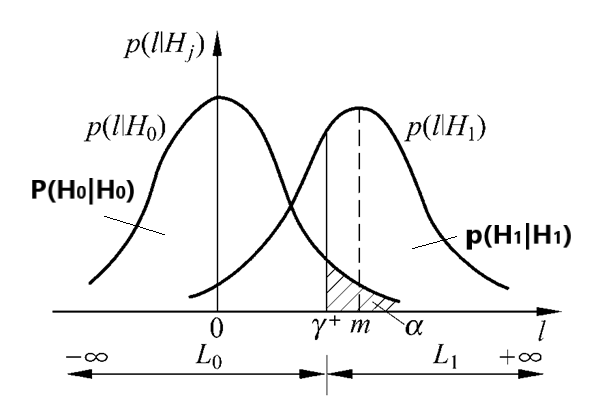
\includegraphics[scale=0.3]{mgt0}
\end{columns}
\end{frame}

\section{贝叶斯准则方法例题11}

\begin{frame}{贝叶斯准则方法例题11}
在二元参量信号的统计检测中,两个假设下的信号分别为:
\begin{align*}
H_0: x&=n  \\
H_1: x&=m+n
\end{align*}
其中, $m$是未知参量, $n$是均值为零,方差为$\sigma_n^2$的高斯白噪声,  试给$m$不同特性参量情况下的最佳信号检测方法。
\end{frame}

\begin{frame}[shrink]{贝叶斯准则方法例题11: 解}
解: 
\begin{align*}
H_0: x&=n\\
H_1: x&=m+n
\end{align*}
\textbf{步骤1: 计算两个似然函数, 构建似然比}\\
由于$n$是高斯分布随机变量, 因此在$H_0$假设下, 观测信号$x$也服从高斯分布,且均值为0, 方差为$\sigma_n^2$; 在$H_1$和给定$m$条件下, 观测信号$x$服从均值为$m$, 方差为$\sigma_n^2$的高斯分布。。
\begin{align*}
p(x|H_0)&=\left(\frac{1}{2\pi\sigma_n^2}\right)^{1/2}\exp\left(-\frac{x^2}{2\sigma_n^2}\right)\\
p(x|m; H_1)&=\left(\frac{1}{2\pi\sigma_n^2}\right)^{1/2}\exp\left(-\frac{(x-m)^2}{2\sigma_n^2}\right)
\end{align*} 
\end{frame}

\begin{frame}[shrink]{贝叶斯准则方法例题11: 解续(1)}
\textbf{步骤2: 形成贝叶斯检测基本表达式}
\begin{align*}
\lambda(x)=\frac{p(x|m; H_1)}{p(x|H_0)}&\mathop{\gtrless}\limits_{H_0}^{H_1}\eta\\
\exp\left(\frac{m}{\sigma_n^2}x-\frac{m^2}{2\sigma_n^2}\right)&\mathop{\gtrless}\limits_{H_0}^{H_1}\eta
\end{align*} 
\textbf{步骤3: 化简, 形成贝叶斯检测判决表达式}
\begin{align*}
\left(\frac{m}{\sigma_n^2}x-\frac{m^2}{2\sigma_n^2}\right)&\mathop{\gtrless}\limits_{H_0}^{H_1}\ln\eta\\
mx&\mathop{\gtrless}\limits_{H_0}^{H_1}\sigma_n^2\ln\eta+\frac{m^2}{2}\mathop{=}^{def}\gamma
\end{align*}
\end{frame}

\begin{frame}[shrink]{贝叶斯准则方法例题11: 解续(2)}
\begin{align*}
mx&\mathop{\gtrless}\limits_{H_0}^{H_1}\sigma_n^2\ln\eta+\frac{m^2}{2}\mathop{=}^{def}\gamma
\end{align*}
\begin{enumerate}
	\item 当$m>0$, 且为确知信号参量时, 似然比检验为
	\[ x\mathop{\gtrless}\limits_{H_0}^{H_1}\frac{\sigma_n^2}{m}\ln\eta+\frac{m}{2}\mathop{=}^{def}\gamma^{+} \]
	\item 当$m<0$, 且为确知信号参量时, 似然比检验为
	\[ x\mathop{\gtrless}\limits_{H_1}^{H_0}-\frac{\sigma_n^2}{|m|}\ln\eta-\frac{|m|}{2}\mathop{=}^{def}\gamma^{-} \]
\end{enumerate} 
\end{frame}

\begin{frame}[shrink]{贝叶斯准则方法例题11: 解续(2)}
\begin{enumerate}
	\setcounter{enumi}{2} %设定起始编号 
	\item 当$m$是随机参量, 且$m\sim\mathcal{N}(0, \sigma_m)$, 其概率密度函数为
	\begin{align*}
	p(m)=\left(\frac{1}{2\pi\sigma_m^2}\right)^{1/2}\exp\left(-\frac{m^2}{2\sigma_m^2}\right)
	\end{align*}
	由例题10得到:
	\begin{align*}
	x^2\mathop{\gtrless}_{H_0}^{H_1}\frac{2\sigma_n^2(\sigma_n^2+\sigma_m^2)}{\sigma_m^2}\left(\ln\eta+\frac{1}{2}\ln\left(1+\frac{\sigma_m^2}{\sigma_n^2}\right)\right)
	\end{align*}
	\item 假设$m_0\le m\le m_1$,其概率密度函数p(m)未知
	似然比检验为:
	\begin{align*}
	mx\mathop{\gtrless}\limits_{H_0}^{H_1}\sigma_n^2\ln\eta+\frac{m^2}{2}
	\end{align*}
	在$m(m_0\le m\le m_1)$取某个值的条件下,采用奈曼-皮尔逊准则来建立判决表达式。
\end{enumerate} 
\end{frame}

\begin{frame}[shrink]{贝叶斯准则方法例题11: 解续(3)}
在$m(m_0\le m\le m_1)$取某个值的条件下,采用奈曼-皮尔逊准则来建立判决表达式。
\begin{enumerate}
	\item[4.1] 若$m_0>0$,判决表示式为
	\begin{align*}
	mx&\mathop{\gtrless}\limits_{H_0}^{H_1}\sigma_n^2\ln\eta+\frac{m^2}{2}\\
    l(x)=x&\mathop{\gtrless}\limits_{H_0}^{H_1}\frac{\sigma_n^2}{m}\ln\eta+\frac{m}{2}\mathop{=}^{def}\gamma^{+} 
	\end{align*}
	\begin{columns}
		\column{0.7\textwidth}
		在$P(H_1|H_0)=\alpha$约束条件下, $\gamma^{+}$由下式确定:
		\[ P(H_1|H_0)=\int_{\gamma^{+}}^{\infty}\left(\frac{1}{2\pi\sigma_n^2}\right)^{1/2}\exp\left(-\frac{l^2}{2\sigma_n^2}\right)dl=\alpha \]
		\column{0.4\textwidth}
		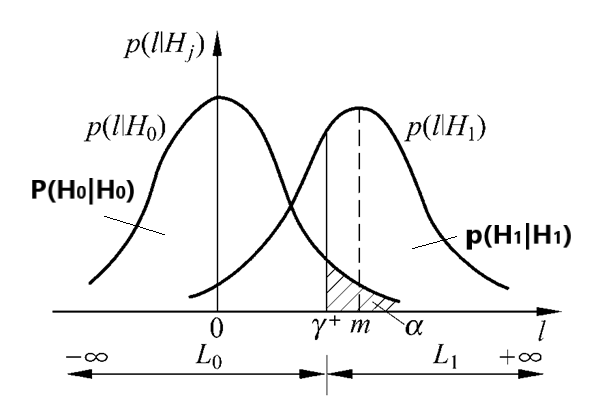
\includegraphics[scale=0.3]{mgt0}
	\end{columns}
\end{enumerate} 
\end{frame}

\begin{frame}[shrink]{贝叶斯准则方法例题11: 解续(4)}
在$m(m_0\le m\le m_1)$取某个值的条件下,采用奈曼-皮尔逊准则来建立判决表达式。
\begin{enumerate}
	\item[4.2] 若$m_1<0$,判决表示式为
	\begin{align*}
	mx&\mathop{\gtrless}\limits_{H_0}^{H_1}\sigma_n^2\ln\eta+\frac{m^2}{2}\\
	l(x)=x&\mathop{\gtrless}\limits_{H_1}^{H_0}-\frac{\sigma_n^2}{|m|}\ln\eta-\frac{|m|}{2}\mathop{=}^{def}\gamma^{-}
	\end{align*}
	\begin{columns}
		\column{0.7\textwidth}
		在$P(H_1|H_0)=\alpha$约束条件下, $\gamma^{-}$由下式确定:
		\[ P(H_1|H_0)=\int_{-\infty}^{\gamma^{-}}\left(\frac{1}{2\pi\sigma_n^2}\right)^{1/2}\exp\left(-\frac{l^2}{2\sigma_n^2}\right)dl=\alpha \]
		\column{0.4\textwidth}
		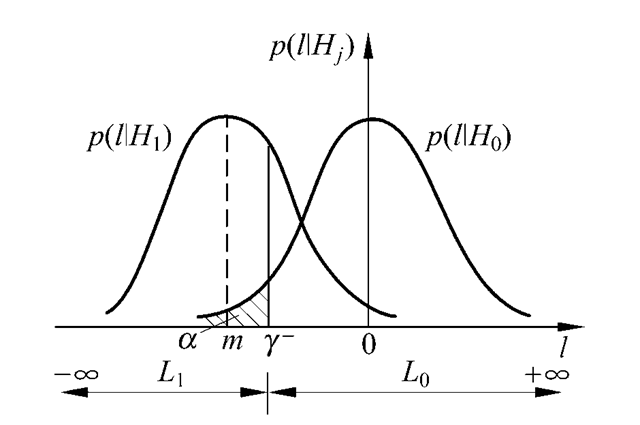
\includegraphics[scale=0.3]{mle0}
	\end{columns}
\end{enumerate} 
\end{frame}

\begin{frame}[shrink]{贝叶斯准则方法例题11: 解续(5)}
在$m(m_0\le m\le m_1)$取某个值的条件下,采用奈曼-皮尔逊准则来建立判决表达式。
\begin{enumerate}
	\item[4.3] 若$m_0>0$或$m_1<0$小结
	\begin{enumerate}
		\item 若$m_0>0$, $m$仅取正值, 则在$P(H_1|H_0)=\alpha$的约束下, $P^{(m)}(H_1|H_1)$是最大的,其一致最大功效检验成立;
		\item 若$m_1<0$, $m$仅取负值, 则在$P(H_1|H_0)=\alpha$的约束下, $P^{(m)}(H_1|H_1)$也是最大的。
	\end{enumerate}
	\begin{columns}
		\column{0.4\textwidth}
		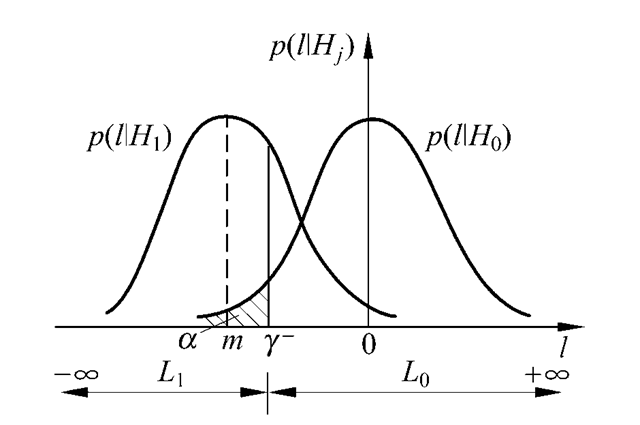
\includegraphics[scale=0.4]{mle0}
		\column{0.4\textwidth}
		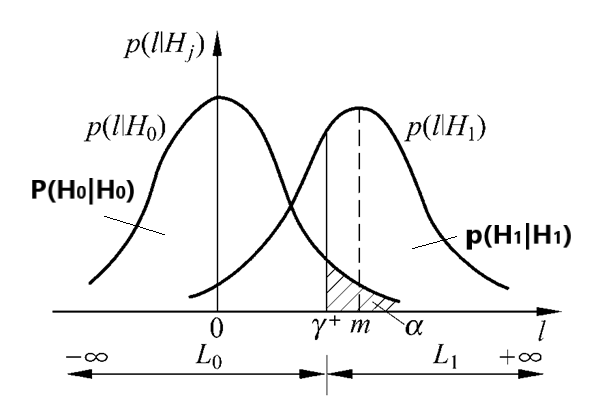
\includegraphics[scale=0.28]{mgt0}
	\end{columns}
\end{enumerate} 
\end{frame}

\begin{frame}[shrink]{贝叶斯准则方法例题11: 解续(6)}
在$m(m_0\le m\le m_1)$取某个值的条件下,采用奈曼-皮尔逊准则来建立判决表达式。
\begin{enumerate}
	\item[4.4] 若$m_0<0,m_1>0$, 即$m$取值可能为正或可能为负的情况下, 无论参量信号的统计检测,按$m$仅取正值设计,还是按$m$仅取负值设计,都有可能在某些$m$值下,   $P^{(m)}(H_1|H_1)$不满足最大的要求。\\
	例如,按$m$取正设计信号检测系统,当$m$为正时,$P^{(m)}(H_1|H_1)$最大, 但当$m$为负时, $P^{(m)}(H_1|H_1)$可能最小。\\
	因此, 这种情况下不能采用奈曼-皮尔逊准则来实际最佳检测系统。
	\begin{columns}
		\column{0.4\textwidth}
		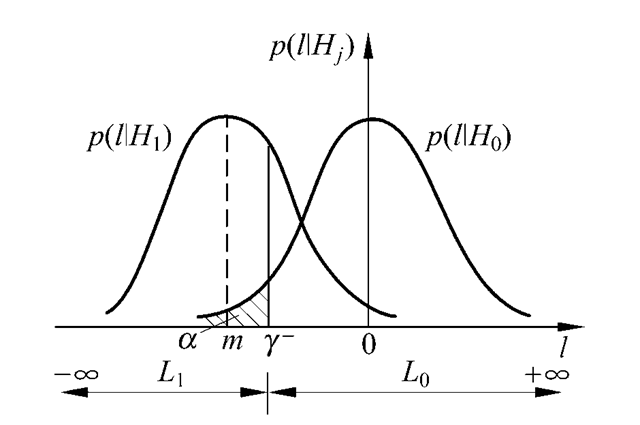
\includegraphics[scale=0.4]{mle0}
		\column{0.4\textwidth}
		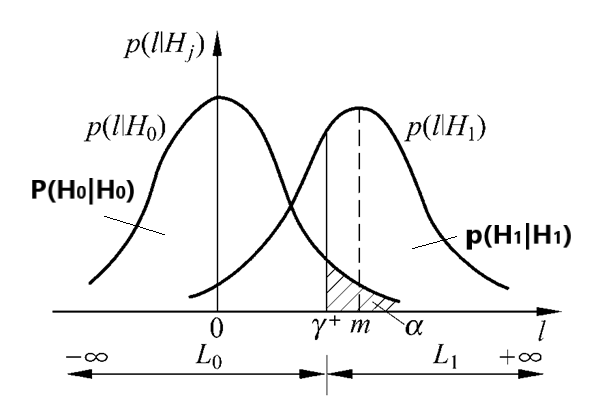
\includegraphics[scale=0.28]{mgt0}
	\end{columns}
\end{enumerate} 
\end{frame}

\begin{frame}[shrink]{贝叶斯准则方法例题11: 解续(6)}
\begin{enumerate}
	\setcounter{enumi}{4} %设定起始编号 
	\item 双边检验\\
	若$m_0<0,m_1>0$, 即$m$取值可能为正或可能为负,奈曼-皮尔逊准则不能保证$P^{(m)}(H_1|H_1)$最大要求。考虑把约束条件$P(H_1|H_0)=\alpha$分成两个$\alpha/2$, 假设$H_1成立$的判决域由两部分组成。判决表示式为
	\[|x|\mathop{\gtrless}_{H_0}^{H_1}\gamma \]
	\begin{columns}
		\column{0.6\textwidth}
		\textcolor{blue}{虽然双边检验比均值$m$假定为正确时的单边检验性能差,但是比均值$m$假定为错误时的单边检验性能要好的多。因此不失为一种好的折中方法。}
		\column{0.3\textwidth}
		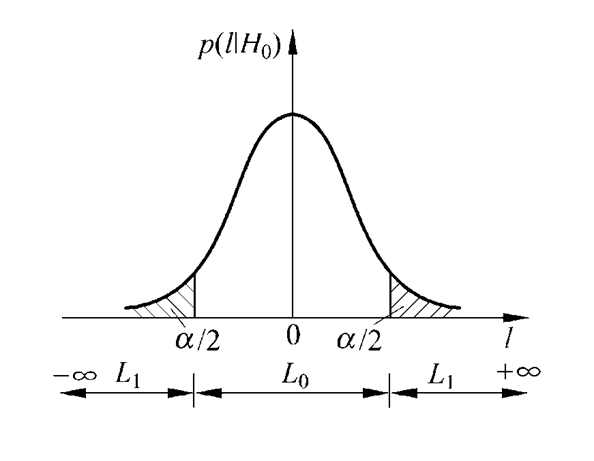
\includegraphics[scale=0.5]{Qd}
	\end{columns}
\end{enumerate} 
\end{frame}

\begin{frame}[shrink]{贝叶斯准则方法例题11: 解续(7)}
\begin{enumerate}
	\setcounter{enumi}{5} %设定起始编号 
	\item 广义似然比检验\\
	\begin{align*}
	&\text{似然函数}\\
	&p(x|m;H_1)=(\frac{1}{2\pi\sigma_n^2})^{1/2}\exp(-\frac{(x-m)^2}{2\sigma_n^2})\\
	&\text{对$m$求偏导,令结果等于零,即} \\
	&\frac{\partial\ln p(x|m;H_1)}{\partial m}|_{m=\widehat{m}_{ml}}=0\\
	&\text{解得单次观测时, $m$的最大似然估计量$\widehat{m}_{ml}=x$, 于是有 }\\
	&p(x|\widehat{m}_{ml};H_1)=(\frac{1}{2\pi\sigma_n^2})^{1/2}\exp(-\frac{(x-\widehat{m}_{ml})^2}{2\sigma_n^2})|_{\widehat{m}_{ml}=x}=(\frac{1}{2\pi\sigma_n^2})^{1/2}\\
	\end{align*}
\end{enumerate} 
\end{frame}

\begin{frame}[shrink]{贝叶斯准则方法例题11: 解续(8)}
\begin{enumerate}
	\setcounter{enumi}{5} %设定起始编号 
	\item 广义似然比检验\\
	\begin{align*}
	&p(x|H_0)=(\frac{1}{2\pi\sigma_n^2})^{1/2}\exp(-\frac{x^2}{2\sigma_n^2})
	&p(x|\widehat{m}_{ml};H_1)=(\frac{1}{2\pi\sigma_n^2})^{1/2}\\
	&\text{代入广义似然比检验中, 有}\\
	&\lambda(x)=\frac{p(x|m; H_1)}{p(x|H_0)}\mathop{\gtrless}_{H_0}^{H_1}\eta\\
	&\lambda(x)=\frac{(\frac{1}{2\pi\sigma_n^2})^{1/2}}{(\frac{1}{2\pi\sigma_n^2})^{1/2}\exp(-\frac{x^2}{2\sigma_n^2})}\mathop{\gtrless}_{H_0}^{H_1}\eta\\
	&\text{化简得判决表示式}
	&x^2\mathop{\gtrless}_{H_0}^{H_1}2\sigma_n^2\ln\eta\mathop{=}^{def}\gamma^2 \implies |x|\mathop{\gtrless}_{H_0}^{H_1}\gamma
	\end{align*}
	\textcolor{blue}{这正是前面讨论过的双边检验。只是前面是从奈曼-皮尔逊准则出发推导得到。而这里是从似然比检验的概念导出的,似然函数$p(x|m;H_1)$中的信号参量$m$由其最大似然估计量$\widehat{m}_{ml}$代换,所以是广义似然比检验。}
\end{enumerate} 
\end{frame}

